\chapter{Практическая часть}

Для реализации аналитического решения ОДУ методом Пикара в контексте данного задания, необходимо определить представление полинома в программе.

Запишем полином в виде массива, где для $i \in \big\{0\big\} \cup \mathbb{N}$ коэффициент одночлена степени $i$ записывается в $i$-ой позиции этого массива. Такая форма хранения многочлена предоставляет быстрый доступ к составляющим его одночленам по их степени.

Обратим внимание, что в рассматриваемой задаче полином каждого последующего приближения содержит одночлен вида $r\cdot{}x^{p + 4}$, где $r$~--- некоторый коэффициент, $p$~--- максимальная степень среди всех одночленов полинома предыдущего приближения. Кроме того, минимальная степень одночлена в любом возможном для данной задачи полиноме равна 3. Следовательно, можно не хранить в массиве коэффициенты тех одночленов, которые никогда не будут содержаться в многочлене. Тогда для вычисления степени $p$ $i$-того одночлена следует использовать следующую формулу:
\begin{equation}
    p = 3 + i \cdot 4
\end{equation}

Теперь необходимо рассмотреть задачи интегрирования и произведения полиномов.

\section{Интегрирование многочлена}
Задача интегрирования полинома это задача интегрирования каждого входящего в его состав одночлена. Имеем:
\begin{equation}
    \int{r \cdot x^n dx} = r \cdot \int{x^n dx} = r \cdot \frac{x^{n + 1}}{n + 1},\quad{}n \ne -1
\end{equation}

\section{Произведение многочленов}
Традиционный алгоритм произведение полиномов имеет $O(n^2)$ асимптотическую трудоёмкость. Скорость такого умножения можно повысить двумя способами:
\begin{itemize}
    \item отбросить одночлены с нулевыми коэффициентами;
    \item производить параллельные вычисления.
\end{itemize}
Описание первого улучшения было приведено выше. Для достижения второго необходимо разбить множество одночленов, из которых состоит, например, первый полином, на $m$ непересекающихся подмножеств, где $m$~--- количество потоков.

Пусть каждый $j$-ый поток вычисляет произведение второго полинома на $k$-ый одночлен первого многочлена, где $j = \overline{0,m-1}$, $k = i + z \cdot m$, $z \in \big\{0\big\} \cup \mathbb{N}$.

$\blacksquare$

Для более быстрого вычисления произведения двух многочленов можно применить метод умножения, основанный на дискретном преобразовании Фурье. Данный метод обычно применяется к целым числам, так как имеет высокую погрешность для чисел с плавающей запятой. Чтобы сделать вывод о допустимости применения такого решения поставленной задачи, реализуем его.

Итак, $DFT(\overrightarrow X)$~--- операция, производящая дискретное преобразование Фурье над вектором чисел $\overrightarrow X$. $InverseDFT(\overrightarrow X_{complex})$~--- обратная операция. Так же $A(\overrightarrow X)$, $B(\overrightarrow X)$~--- некоторые полиномы. Тогда:
\begin{flalign*}
    &
    (A \cdot B)(\overrightarrow X) = A(\overrightarrow X) \cdot B(\overrightarrow X)
  \\&
  DFT((A \cdot B)(\overrightarrow X)) = DFT(A(\overrightarrow X)) \cdot DFT(B(\overrightarrow X))
  \\&
  (A \cdot B)(\overrightarrow X) = InverseDFT(DFT(A(\overrightarrow X)) \cdot DFT(B(\overrightarrow X)))
    &
\end{flalign*}
Важно уточнить, что векторы $A(\overrightarrow X)$, $B(\overrightarrow X)$ нужно дополнить нулями так, чтобы $len((A \cdot B)(\overrightarrow X)) = len(A(\overrightarrow X)) = len(B(\overrightarrow X))$, где $len(\vec v)$~--- операция получения длины некоторого вектора $\vec v$.

\section{Инструменты реализации}

Для реализации рассматриваемой задачи используется язык программирования C++.

В целях проведения параллельных вычислений используется библиотека pthread.

Задача выполнения метода Пикара при высоких приближениях требует тип данных, реализующий числа с плавающей точкой с множественной точностью. Для этого применяется библиотека mpfr.

Для вычисления $DFT$ используется быстрое преобразование Фурье. Данный метод реализован в библиотеке Eigen.

\section{Реализация}
В листингах~\ref{picard},~\ref{mtpicard},~\ref{fftpicard} приведён текст различных реализаций методов Пикара.
\begin{lstlisting}[caption={Метод Пикара},label=picard]
class Picard : public APicard
{
public:
    Picard();
    ~Picard();

    void computePol(int approx) override;
    double operator()(double x) override;
    double operator()(double x, int approx) override;

    static const int precision = 200;

    using Real = mpfr::real<precision>;

protected:
    void allocatePols(int maxApprox);

    static inline Real pow(const Real &r, int p)
    { return mpfr::pow(r, p); }

    int approx;
    long long *polLens;
    Real **polynomials;
};

// Вычисление полинома
void Picard::computePol(int approx)
{
    Real *squared;
    Real *polynomial;
    long long curLen = 1;
    long long sqrLen;

    allocatePols(approx);

    squared = new Real[polLens[approx - 1]];
    polynomial = new Real[polLens[approx - 1]];
    polynomial[0] = 1.0 / 3;

    for (int idx = 0; idx < approx; ++idx)
    {
        for (long long i = 0; i < curLen; ++i)
            polynomials[idx][i] = polynomial[i];

        sqrLen = curLen << 1;
        for (long long i = 0; i < sqrLen; i++)
            squared[i] = 0;

        for (long long i = 0; i < curLen; i++)
            for (long long j = 0; j < curLen; j++)
                squared[i + j + 1] += polynomial[i] *
                                      polynomial[j] /
                                      ((int)(i + j + 1) * 4 + 3);
        squared[0] = 1.0 / 3;

        std::swap(polynomial, squared);
        curLen = sqrLen;
    }

    delete[] squared;
    delete[] polynomial;
}

// Подстановка значения в полином
double Picard::operator()(double x, int approx)
{
    if (!polynomials)
        return 0;
    if (approx > this->approx)
        return 0;

    Real res = 0;

    for (int i = 0; i < polLens[approx - 1]; i++)
        res += polynomials[approx - 1][i] * pow(Real(x), i * 4 + 3);

    return res;
}
\end{lstlisting}
\begin{lstlisting}[caption={Параллелизированный метод Пикара},label=mtpicard]
class MTPicard : public Picard
{
public:
    void computePol(int approx) override;
};

void MTPicard::computePol(int approx)
{
    Real *squared;
    Real *polynomial;
    long long curLen = 1;
    long long sqrLen;

    allocatePols(approx);
    squared = new Real[polLens[approx - 1]];
    polynomial = new Real[polLens[approx - 1]];
    polynomial[0] = 1.0 / 3;

    std::vector<std::thread> threads;

    for (int idx = 0; idx < approx; ++idx)
    {
        for (long long i = 0; i < curLen; ++i)
            polynomials[idx][i] = polynomial[i];

        sqrLen = curLen << 1;
        for (long long i = 0; i < sqrLen; i++)
            squared[i] = 0;

        for (int i = 1; i <= THREADS_QTY; i++)
            threads.push_back(std::thread(
                        &::squarePolPart,
                        squared, i, sqrLen, THREADS_QTY,
                        polynomial));

        for (std::thread &thread: threads)
            thread.join();

        squared[0] = 1.0 / 3;

        std::swap(polynomial, squared);
        curLen = sqrLen;
        threads.clear();
    }

    delete[] squared;
    delete[] polynomial;
}

static void squarePolPart(
        mmlabs::Picard::Real *squared,
        long long begin, long long end, long long step,
        mmlabs::Picard::Real *polynomial
        )
{
    for (long long i, idx = begin; idx < end; idx += step)
    {
        i = idx - 1;

        do
            squared[idx] += polynomial[i] *
                            polynomial[idx - 1 - i] /
                            ((int)idx * 4 + 3);
        while (i--);
    }
}
\end{lstlisting}
\begin{lstlisting}[caption={Метод Пикара, основанный на быстром преобразовании Фурье},label=fftpicard]
template<typename TComplex>
class FFT;

class FFTPicard : public Picard
{
public:
    FFTPicard();
    ~FFTPicard();

    void computePol(int approx) override;

    using Complex = std::complex<Real>;

private:
    FFT<Complex> *fft;
};

void FFTPicard::computePol(int approx)
{
    int sqrLen = 1;
    Complex *polynomialComplex;
    Complex *integratedComplex;

    allocatePols(approx);
    polynomialComplex = new Complex[polLens[approx - 1]];
    integratedComplex = new Complex[polLens[approx - 1]];
    polynomialComplex[0] = 1.0 / 3;

    fft->setMaxVectorSize(polLens[approx - 1]);

    for (int idx = 0; idx < approx; ++idx)
    {
        for (long long i = 0; i < polLens[idx]; ++i)
            polynomials[idx][i] = polynomialComplex[i].real();

        sqrLen <<= 1;

        (*fft)(polynomialComplex, sqrLen, false);
        for (long long i = 0; i < sqrLen; ++i)
            polynomialComplex[i] *= polynomialComplex[i];
        (*fft)(polynomialComplex, sqrLen, true);

        for (long long i = 0; i < sqrLen - 1; ++i)
            integratedComplex[i + 1] = polynomialComplex[i] /
                                       Complex((int)(i + 1) * 4 + 3);

        integratedComplex[0] = 1.0 / 3;
        std::swap(integratedComplex, polynomialComplex);
    }

    delete[] polynomialComplex;
    delete[] integratedComplex;
}
\end{lstlisting}

В листинге~\ref{exeuler} приведён текст реализации явного метода Эйлера.
\begin{lstlisting}[caption={Явный метод Эйлера},label=exeuler]
double explicitMethod(double x, double h)
{
    double res = 0;
    double x0 = h;

    while (x0 < x + h)
    {
        res += h * (x0 * x0 + res * res);
        x0 += h;
    }

    return res;
}
\end{lstlisting}

В листинге~\ref{imeuler} приведён текст реализации неявного метода Эйлера.
\begin{lstlisting}[caption={Неявный метод Эйлера},label=imeuler]
double implicitMethod(double x, double h)
{
    double D;
    double res = 0;
    double x0 = h;

    while (x0 < x + h)
    {
        D = 1 - 4 * h * (h * x0 * x0 + res);

        if (D >= 0)
            res = (1 - ::sqrt(D)) / 2 / h;

        x0 += h;
    }

    return res;
}
\end{lstlisting}

\section{Примеры работы}
На рисунках~\ref{img:mtpicard},~\ref{img:fftpicard} изображены примеры реализованной программы. В первом случае используется параллеллизированный метод Пикара, во втором~--- метод Пикара, основанный на быстром преобразовании Фурье.
\begin{figure}[H]
    \caption{Параллелизированный метод Пикара}\label{img:mtpicard}
    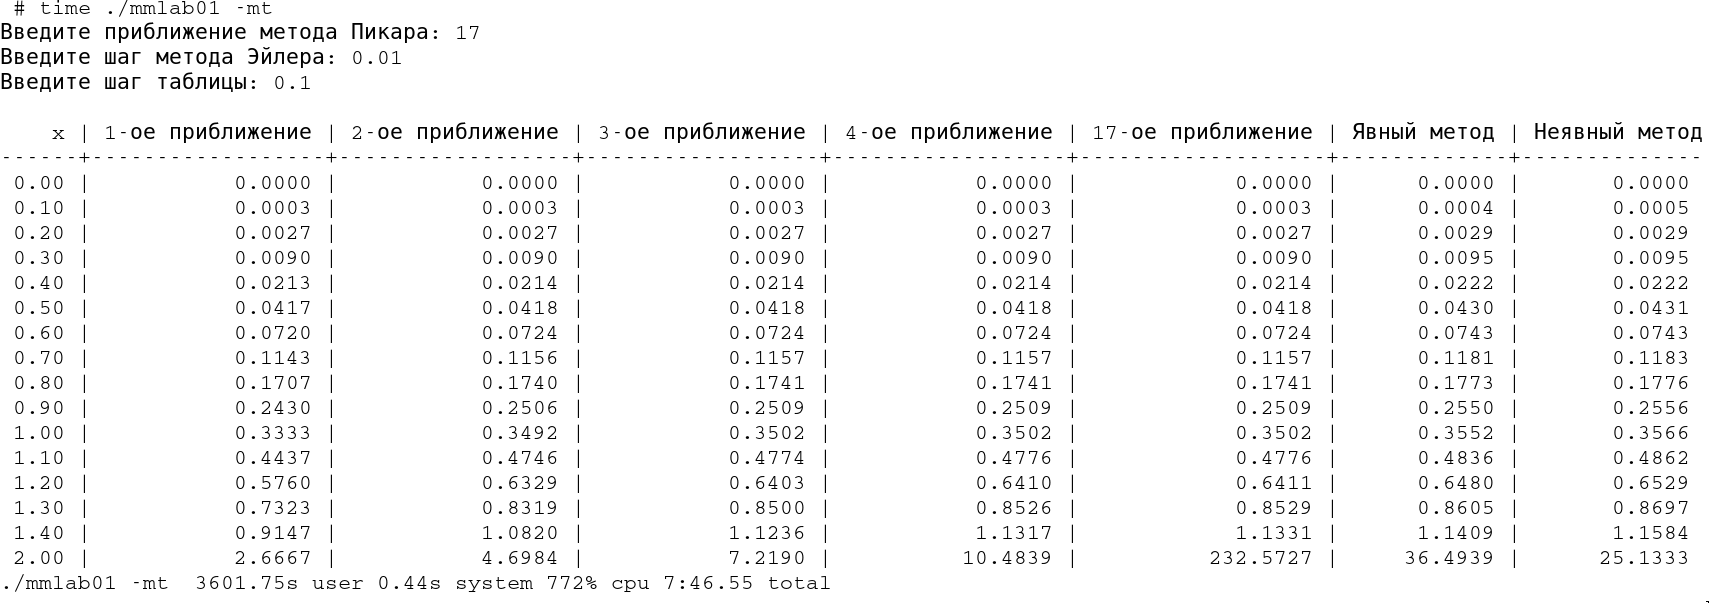
\includegraphics[scale=0.27]{images/mtpicard.png}
\end{figure}
\begin{figure}[H]
    \caption{Метод Пикара, основанный на быстром преобразовании Фурье}\label{img:fftpicard}
    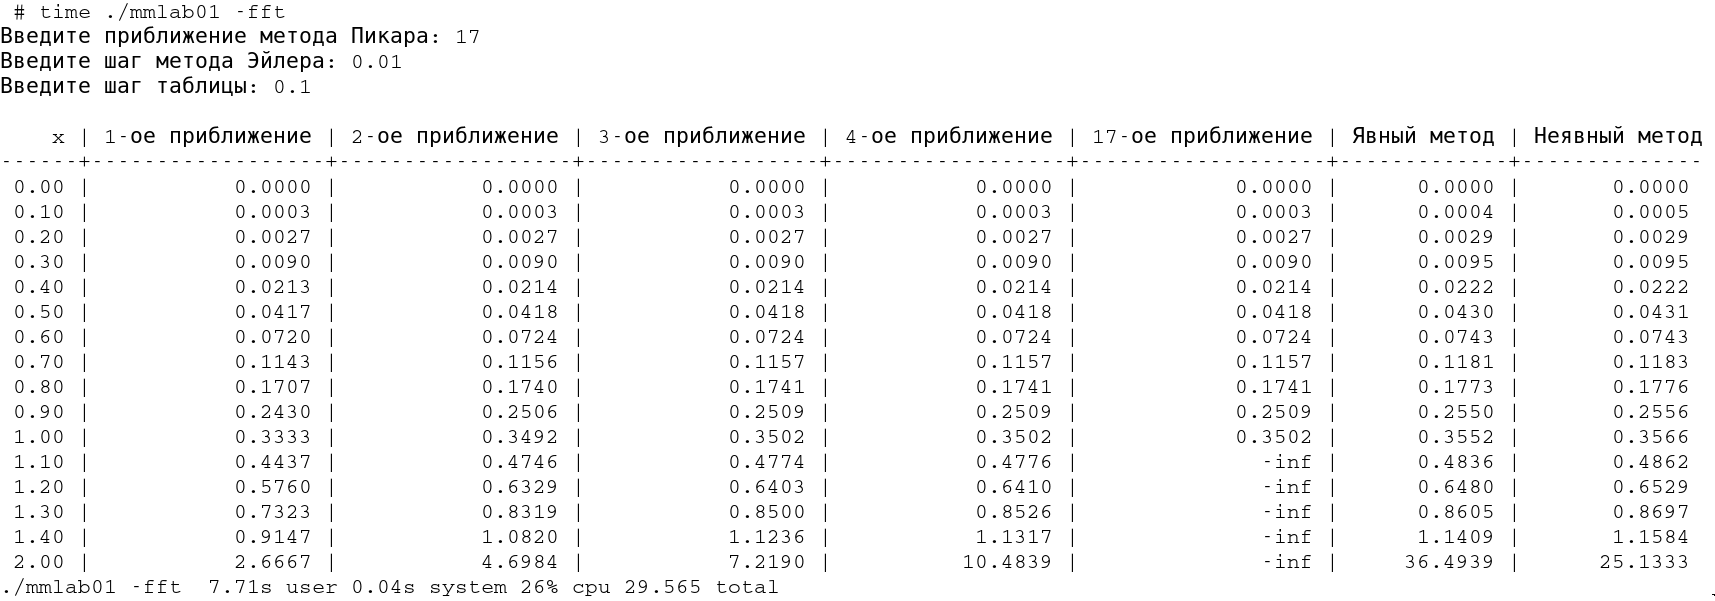
\includegraphics[scale=0.27]{images/fftpicard.png}
\end{figure}
Как видно, высокая погрешность быстрого преобразования Фурье не позволяет использовать этот метод для реализации метода Пикара.

\section{Ответы на контрольные вопросы}

\subsection{Укажите интервалы значений аргумента, в которых можно считать решением заданного уравнения каждое из первых 4-х  приближений Пикара. Точность результата оценивать до второй цифры после запятой. Объяснить свой ответ.}

Чтобы проверить, сходится ли $n$-ое приближение Пикара к точному, нужно вычислить следующее. Если $y_n$ и $y_{n+1}$ равны с точностью до некоторого знака (в данном случае до второго), то $n$-ое приближение можно считать решением заданного уравнения.

Необходимое условие можно задать таким образом:
\begin{equation*}
    y_{n + 1}(x) - y_{n}(x) < 0.01
\end{equation*}

Для первых четырёх приближений имеем:

\begin{equation}\label{eq:picard1}
    y_2(x) - y_1(x) < 0.01
\end{equation}
\begin{equation}\label{eq:picard2}
    y_3(x) - y_2(x) < 0.01
\end{equation}
\begin{equation}\label{eq:picard3}
    y_4(x) - y_3(x) < 0.01
\end{equation}
\begin{equation}\label{eq:picard4}
    y_5(x) - y_4(x) < 0.01
\end{equation}

Для решения этих неравенств была реализована программа, текст который представлен в листинге~\ref{lst:picardtest}.
\begin{lstlisting}[caption={Поиск интервалов},label={lst:picardtest}]
int main()
{
    std::vector<double> v;
    mmlabs::MTPicard picard;

    int maxApprox = 4;

    int p = 2;
    int n = 3;
    double eps = 1 * pow(10.0, -p);
    double step = 1 * pow(10.0, -n);

    picard.computePol(maxApprox + 1);

    for (int i = 1; i <= maxApprox; ++i)
    {
        v.push_back(estimateMaxX(picard, i, i + 1, step, eps));
        printf("x_%d <= %.*lf\n", i, n, *v.rbegin());
    }
    printf("\n");

    printf("x <= %.*lf\n", n, *std::min_element(v.begin(), v.end()));

    return 0;
}

double estimateMaxX(mmlabs::MTPicard &picard,
                    int approx1, int approx2,
                    double step, double eps)
{
    double x = 0;
    double y1, y2;

    while (fabs((picard(x, approx2)) - (y1 = picard(x, approx1))) < eps)
        x += step;

    return x - step;
}
\end{lstlisting}

На рисунке~\ref{img:answer1} приведён результат работы этой программы.
\begin{figure}[H]
    \centering
    \caption{Поиск $u(2)$}\label{img:answer1}
    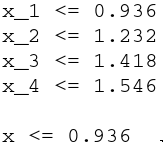
\includegraphics[scale=0.5]{images/picard_test.png}
\end{figure}

Таким образом, при $\underline{\underline{x \in [0, 0.936]}}$ решением заданного уравнения можно считать каждое из первых 4-х приближений Пикара.

\subsection{Пояснить, каким образом можно доказать правильность полученного результата при фиксированном значении аргумента в численных методах.}\label{ans2}
Численные методы зависят от шага. Чем меньше шаг~--- тем точнее решение. Чтобы доказать правильность полученного результата с точностью до $n$-ой цифры после запятой, нужно уменьшать шаг до тех пор, пока результаты для двух крайних шагов не перестанут отличаться с точностью до $n$-ой цифры после запятой.

\subsection{Из каких соображений выбирался корень уравнения в неявном методе?}
В неявном методе выбирается минимальный корень для того, чтобы минимизировать накапливаемую ошибку и, тем самым, повысить точность.

\subsection{Каково значение функции при $x=2$, т.е. привести значение $u(2)$.}
Для поиска $u(2)$ используем явный метод Эйлера. С учётом ответа на вопрос~\ref{ans2} была реализована программа, текст которой приведён в листинге~\ref{euler_test}.
\begin{lstlisting}[caption={Поиск $u(2)$}, label={euler_test}]
int main()
{
    const double EPS = 1e-2;

    double y;
    double y_next;

    double x = 2;
    double h = 1e-1;

    int h_len = 7;
    int h_frac_len = 1;
    int y_len = 8;
    int y_frac_len = 4;

    char hrule[256] = {};
    memset(hrule, '-', sizeof(hrule) - 1);

    printf("Явный метод Эйлера, x = %.1lf\n", x);

    printf(" %*s | %*s \n", h_len, "h", y_len, "y");
    printf("-%.*s-+-%.*s-\n", h_len, hrule, y_len, hrule);

    y_next = mmlabs::EulerMethod::explicitMethod(x, h);

    do
    {
        y = y_next;

        printf(" %*.*e | %*.*lf \n",
               h_len, h_frac_len, h, y_len, y_frac_len, y);

        h /= 10;
        y_next = mmlabs::EulerMethod::explicitMethod(x, h);
    }
    while (fabs(y_next - y) >= EPS);

    printf(" %*.*e | %*.*lf \n",
           h_len, h_frac_len, h, y_len, y_frac_len, y_next);

    return 0;
}
\end{lstlisting}

Результат работы этой программы приведён на рисунке~\ref{img:answer4}.
\begin{figure}[H]
    \centering
    \caption{Поиск интервалов}\label{img:answer4}
    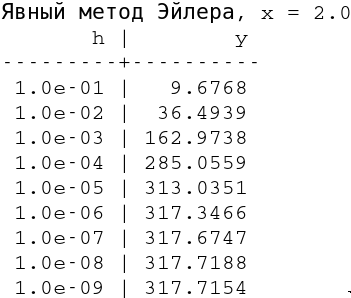
\includegraphics[scale=0.5]{images/euler_test.png}
\end{figure}

В полученной таблице последний и предпоследний результаты равны с точностью до второго знака после запятой. Таким образом, $\underline{\underline{u(2) \approx 317.72}}$.

